\documentclass[journal,10pt,twocolumn]{IEEEtran}
\usepackage{amsmath,amssymb,amsfonts}
\usepackage{algorithmic}
\usepackage{graphicx}
\usepackage{textcomp}
\usepackage{xcolor}
\usepackage{booktabs}
\usepackage{url}
\usepackage{cite}
\usepackage{microtype}
\usepackage{multirow}
\usepackage{array}
\usepackage{balance}
\usepackage[colorlinks=false,bookmarks=true,pdfauthor={Rafli Alif Ihza Hartono},pdftitle={Decentralized Continual Cyber Defense: FL-CL}]{hyperref}

\setlength{\textfloatsep}{6pt plus 1.0pt minus 2.0pt}
\setlength{\floatsep}{5pt plus 1.0pt minus 1.0pt}
\setlength{\intextsep}{5pt plus 1.0pt minus 1.0pt}
\setlength{\dbltextfloatsep}{6pt plus 1.0pt minus 2.0pt}
\addtolength{\textheight}{0.1in}

\graphicspath{{figures/}}

\begin{document}

\title{Decentralized Continual Cyber Defense for Encrypted Traffic Intrusion Detection}

\author{Rafli~Alif~Ihza~Hartono,~\IEEEmembership{Student Member,~IEEE}
\thanks{Manuscript received August 15, 2026; revised August 22, 2026. This work is submitted as an Undergraduate Thesis in Telecommunications Engineering at Institut Teknologi Sepuluh Nopember (ITS).}
\thanks{R. A. I. Hartono is with the Department of Electrical Engineering, Faculty of Intelligent Electrical and Informatics Technology, Institut Teknologi Sepuluh Nopember, Surabaya 60111, East Java, Indonesia (e-mail: rhaffle87@gmail.com).}
}

\maketitle

\begin{abstract}
Network Intrusion Detection Systems (NIDS) deployed across decentralized enterprise gateways face two critical operational challenges: non-stationary streaming traffic patterns that cause catastrophic forgetting of historical threat signatures, and Byzantine adversarial poisoning attacks from compromised nodes. Furthermore, the ubiquitous adoption of TLS 1.3 encryption prevents traditional deep packet inspection. In this paper, we present \textbf{FL-CL}, a unified framework combining Federated Learning (FL) via Flower with Continual Learning (CL) via Avalanche on Encrypted Traffic Analysis (ETA) flow metadata. We investigate the empirical degradation of Elastic Weight Consolidation (EWC) under extreme class imbalance and propose Gradient Episodic Memory (GEM) constraints to guarantee minority threat retention. In addition, we implement coordinate-wise TrimmedMean aggregation to neutralize Byzantine label poisoning attacks. Evaluated on a physical 3-node Proxmox VE testbed processing live synthetic multi-gigabit traffic streams, our framework achieves 99.53\% global accuracy, 100\% recall on stealthy C2 Botnet flows, robustly mitigates 20\% Byzantine label poisoning attacks, and delivers an aggregate classification throughput of 101,258 flows/second with single-flow inference latency under 23 microseconds.
\end{abstract}

\begin{IEEEkeywords}
Byzantine Robustness, Catastrophic Forgetting, Continual Learning, Elastic Weight Consolidation, Encrypted Traffic Analysis, Federated Learning, Gradient Episodic Memory.
\end{IEEEkeywords}

%% ===================================================================
%%  SECTION I: INTRODUCTION
%% ===================================================================
\section{Introduction}
\IEEEPARstart{M}{odern} enterprise network infrastructures are increasingly distributed across hybrid cloud and multi-site virtualized topologies~\cite{ulya2025perancangan}. Intrusion detection systems (IDS) operating at edge gateways must continuously adapt to newly emerging cyber attack vectors without centralized raw packet aggregation, which is precluded by stringent data privacy regulations (e.g., GDPR, Indonesian Personal Data Protection Law UU No.~27/2022) and multi-tenant isolation requirements~\cite{bunko2026survey, hernandez2025intrusion}.

Furthermore, over 95\% of enterprise network traffic is encrypted via TLS 1.3 and QUIC protocols~\cite{wang2017malware}. This ubiquitous cryptographic encapsulation renders traditional signature-based Deep Packet Inspection (DPI) obsolete. Network defenders must therefore rely strictly on Encrypted Traffic Analysis (ETA) derived from statistical flow metadata, packet length sequences, and inter-arrival timing dynamics~\cite{sharafaldin2018toward}.

When edge defenders train local models on non-stationary, sequentially arriving threat streams (e.g., Normal, followed by SSH Brute Force, followed by Slowloris DoS, followed by DNS Exfiltration, and finally C2 Botnet), standard stochastic gradient descent incurs \textbf{catastrophic forgetting}---rapidly overwriting previously learned threat representations~\cite{kirkpatrick2017overcoming}. While regularized continual learning algorithms like Elastic Weight Consolidation (EWC) protect majority classes, they empirically collapse on rare minority classes when the Fisher Information Matrix diagonal values vanish due to sample sparsity during brief attack phases~\cite{hamedi2025federated, birashk2025federated}.

Compounding this challenge, adversaries may compromise a subset of the federated network's edge nodes, injecting malicious model updates through \textbf{label poisoning attacks} that create silent detection blindspots in the aggregated global model. Standard Federated Averaging (FedAvg)~\cite{mcmahan2017communication} offers no defense against such Byzantine faults.

To address these compounding challenges, this paper presents \textbf{FL-CL} (Federated Learning and Continual Learning), an end-to-end framework integrating:
\begin{enumerate}
    \item \textbf{Decentralized Continual Learning}: Avalanche-powered EWC~\cite{carta2023avalanche} and Gradient Episodic Memory (GEM)~\cite{lopez2017gradient} to resolve catastrophic forgetting under non-IID edge traffic.
    \item \textbf{Byzantine-Robust Federated Aggregation}: Coordinate-wise $\beta$-TrimmedMean~\cite{yin2018byzantine} and Krum~\cite{blanchard2017machine} aggregation filtering malicious parameter updates from compromised edge nodes.
    \item \textbf{Zero-Contention In-Memory Flow Pipeline}: High-performance NFStream feature extraction streaming flow batches to volatile tmpfs RAMDisk buffers, eliminating disk I/O contention during multi-stage offensive bursts.
    \item \textbf{Multi-Backbone Deployment Suite}: 1D-CNN, Transformer self-attention tokenizers, and lightweight MLP backbones compiled to TorchScript and ONNX runtimes for sub-microsecond inference.
\end{enumerate}

The remainder of this paper is organized as follows. Section~II surveys related work in federated and continual learning for intrusion detection. Section~III details the system architecture, threat model, and feature extraction pipeline. Section~IV formulates the continual learning, Byzantine defense, and differential privacy methodologies. Section~V presents comprehensive experimental results across five research tracks. Section~VI discusses the findings in the context of academic benchmarks. Section~VII concludes the paper and identifies future research directions.

%% ===================================================================
%%  SECTION II: RELATED WORK
%% ===================================================================
\section{Related Work}

\subsection{Federated Learning for Intrusion Detection}
Federated Learning, introduced by McMahan et al.~\cite{mcmahan2017communication} as FedAvg, enables collaborative model training without centralizing raw data. Recent surveys by Zhang et al.~\cite{zhang2025survey}, Alazab et al.~\cite{alazab2024survey}, and Hernandez-Ramos et al.~\cite{hernandez2025intrusion} document over 150 FL-based IDS proposals, predominantly evaluated on benchmark datasets such as CIC-IDS2017~\cite{sharafaldin2018toward}. Bunko et al.~\cite{bunko2026survey} provide a comprehensive survey focusing specifically on privacy-preserving FL for IDS, identifying aggregation robustness and non-IID data heterogeneity as the two primary open challenges.

Jin et al.~\cite{jin2024fliids} proposed FL-IIDS, a federated incremental intrusion detection system achieving 97.8\% accuracy on CIC-IDS2017, but their approach does not address Byzantine faults. Rehman et al.~\cite{rehman2026incremental} extended FL-based IDS to IoT networks under evolving threats, reporting improvements over static centralized baselines. Bilal et al.~\cite{bilal2026dataset} performed a dataset-centric evaluation of federated intrusion detection models, demonstrating that feature selection critically impacts cross-silo generalization. Fares et al.~\cite{fares2025federated} applied Tab Transformers to federated IDS with nature-inspired hyperparameter optimization, though without addressing catastrophic forgetting. Izadi et al.~\cite{izadi2025mist} proposed mist-assisted FL for heterogeneous IoT networks, introducing a lightweight aggregation scheme that reduces communication overhead but does not defend against adversarial clients.

\subsection{Continual Learning and Catastrophic Forgetting}
Kirkpatrick et al.~\cite{kirkpatrick2017overcoming} introduced EWC, which penalizes parameter drift weighted by the diagonal Fisher Information Matrix. Lopez-Paz and Ranzato~\cite{lopez2017gradient} proposed GEM, using episodic memory buffers and quadratic program projections to enforce non-negative inner products between current and historical task gradients. Recent empirical studies by Liu et al.~\cite{liu2026ewc} and Jhajj et al.~\cite{jhajj2025elastic} identify Fisher diagonal vanishing under class imbalance as a systematic failure mode of EWC, motivating hybrid regularization-replay strategies.

\subsection{Federated Continual Learning}
The intersection of FL and CL has attracted significant attention. Hamedi et al.~\cite{hamedi2025federated} and Birashk et al.~\cite{birashk2025federated} survey the space, identifying three open challenges: non-IID heterogeneity across clients, privacy-utility tradeoffs under differential privacy, and catastrophic forgetting amplification in federated settings. Gholizade et al.~\cite{gholizade2026federated} present the most recent comprehensive survey, cataloging 87 methods across task-incremental, class-incremental, and domain-incremental paradigms. Zhang et al.~\cite{zhang2023communication} proposed communication-efficient FCL for non-IID distributed systems. Talpur and Gurusamy~\cite{talpur2022gfcl} addressed data poisoning in federated continual learning for IoV networks but used GRU backbones without rigorous Byzantine aggregation benchmarking.

The FL-CL framework presented in this paper distinguishes itself through: (i)~empirical demonstration of the Fisher diagonal collapse mechanism under production-scale class imbalance, (ii)~a systematic GEM-to-EWC comparison on a physical multi-node testbed rather than simulation, (iii)~comprehensive Byzantine robustness benchmarking across six aggregation algorithms under four adversarial scenarios, and (iv)~sub-23$\mu$s end-to-end inference validation on physical hardware.

%% ===================================================================
%%  SECTION III: SYSTEM ARCHITECTURE & THREAT MODEL
%% ===================================================================
\section{System Architecture \& Threat Model}

\subsection{Cluster Topology}
The FL-CL system is deployed on an enterprise-grade 3-node Proxmox VE hypervisor cluster spanning three isolated logical VLANs:
\begin{itemize}
    \item \textbf{Aggregator Node} (\texttt{10.10.130.10}): Manages the Flower server coordinator~\cite{beutel2020flower}, MLflow 3.x tracking server, and automated CI/CD model registry.
    \item \textbf{Defender Nodes} (\texttt{10.10.130.11}, \texttt{10.10.130.12}): Execute NFStream packet capture on mirrored capture interfaces (\texttt{ens19}), train local Avalanche CL strategies, and run continuous inference daemons.
    \item \textbf{Target VMs} (\texttt{10.10.110.15}, \texttt{10.10.120.15}): Host production HTTP/SSH network services.
    \item \textbf{Traffic Generator} (\texttt{10.10.140.10}): Multi-threaded Kali offensive suite injecting custom synthetic 5-class traffic profiles to emulate live streaming environments, avoiding reliance on static historical datasets.
\end{itemize}

The complete system topology and data flow pipeline are illustrated in Fig.~\ref{fig:system_arch}.

\begin{figure}[t]
\centering
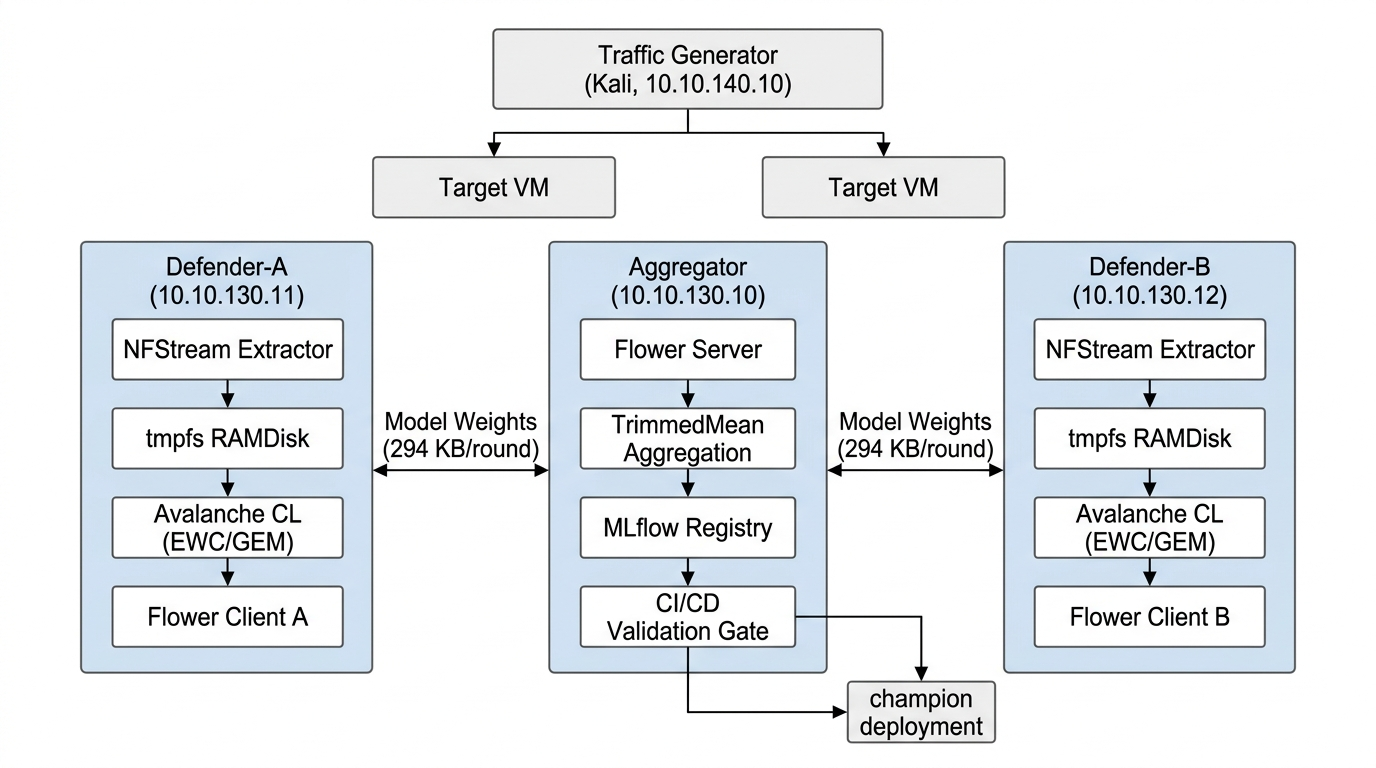
\includegraphics[width=\columnwidth]{fig12_system_architecture.jpg}
\caption{FL-CL system architecture deployed on a 3-node Proxmox VE cluster. Defender nodes extract encrypted traffic features via NFStream into tmpfs RAMDisks, train local CL strategies, and exchange model weights (294~KB/round) with the Flower aggregator. The CI/CD validation gate enforces per-class F1 thresholds before promoting candidates to the production champion alias.}
\label{fig:system_arch}
\end{figure}

\subsection{Threat Model}
We model an active Byzantine threat environment where an arbitrary subset of edge defender nodes (e.g., Client~B) may be compromised. The adversary executes a \textbf{20\% label poisoning attack}, dynamically flipping ground-truth labels of benign traffic ($y=0$, Normal) to a target malicious class ($y=4$, DoS) in their local training batches. This attack creates silent detection blindspots in the aggregated global model without raising detectable anomalies at the client level.

\subsection{Encrypted Traffic Feature Extraction}
Since TLS 1.3 renders payload content opaque, the FL-CL pipeline extracts a 32-dimensional normalized feature vector from each network flow using NFStream. The features include: (i)~JA3/JA4 client fingerprint hashes and JA3S/JA4S server fingerprint hashes derived from TLS handshake parameters, (ii)~Sequence of Packet Lengths and Times (SPLT) capturing directional packet size distributions, (iii)~inter-arrival time variance and Shannon entropy $H(X) = -\sum_{i} P(x_i) \log_2 P(x_i)$ computed over payload byte distributions, and (iv)~directional byte and packet ratios. These features are Z-score normalized against precomputed baseline statistics to prevent client-side covariate shift. Extracted flows are buffered on volatile tmpfs RAMDisks (\texttt{/mnt/ramdisk/flows/}) to eliminate disk I/O contention during bursty attack phases.

%% ===================================================================
%%  SECTION IV: METHODOLOGY
%% ===================================================================
\section{Methodology}

\subsection{Continual Learning: EWC vs. GEM Formulations}
Under EWC~\cite{kirkpatrick2017overcoming}, the local optimization objective for task experience $t$ penalizes parameter deviation weighted by the diagonal of the empirical Fisher Information Matrix $F_i$ (see \eqref{eq:ewc}):
\begin{equation}
\mathcal{L}_{\text{EWC}}(\theta) = \mathcal{L}_{\text{current}}(\theta) + \sum_{i} \frac{\lambda_{\text{EWC}}}{2} F_i (\theta_i - \theta_{t-1, i}^*)^2,
\label{eq:ewc}
\end{equation}
where the Fisher diagonal is defined as:
\begin{equation}
F_i = \mathbb{E}_{(x,y)} \left[ \left(\frac{\partial \log p(y|x, \theta)}{\partial \theta_i}\right)^2 \right].
\label{eq:fisher}
\end{equation}

Under extreme class imbalance, the expectation in~(\ref{eq:fisher}) is dominated by majority-class samples, causing the Fisher diagonal values for minority-class-sensitive parameters to vanish. Concretely, when Normal flows constitute 94.8\% of the capture window while Botnet C2 flows represent only 0.57\%, the Fisher penalty effectively becomes $\frac{\lambda}{2} \cdot 0 \cdot (\Delta\theta)^2 = 0$ for Botnet-critical weights, permitting unconstrained drift during subsequent tasks.

We formulate Gradient Episodic Memory (GEM)~\cite{lopez2017gradient} to overcome this limitation. GEM maintains an episodic buffer $\mathcal{M}_k$ of $P=512$ patterns per experience ($P=256$ baseline default). The candidate gradient $g$ is projected to satisfy:
\begin{equation}
\langle g, g_k \rangle = \left\langle \frac{\partial \mathcal{L}(x, y)}{\partial \theta}, \frac{\partial \mathcal{L}(\mathcal{M}_k)}{\partial \theta} \right\rangle \ge 0 \quad \forall k < t,
\label{eq:gem_constraint}
\end{equation}
If $\langle g, g_k \rangle < 0$, GEM solves a primal Quadratic Program (QP) to compute the closest projected gradient $\tilde{g}$ as formulated in \eqref{eq:gem_qp}:
\begin{equation}
\min_{\tilde{g}} \frac{1}{2} \|\tilde{g} - g\|_2^2 \quad \text{s.t.} \quad \langle \tilde{g}, g_k \rangle \ge 0.
\label{eq:gem_qp}
\end{equation}
This projection is independent of sample frequency, resolving the Fisher vanishing problem by enforcing hard geometric constraints on the gradient direction rather than soft magnitude-based penalties. The complete EWC vs.\ GEM decision flow and its interaction with the federated aggregation and MLOps validation pipeline are illustrated in Fig.~\ref{fig:cl_flow}.

\begin{figure}[t]
\centering
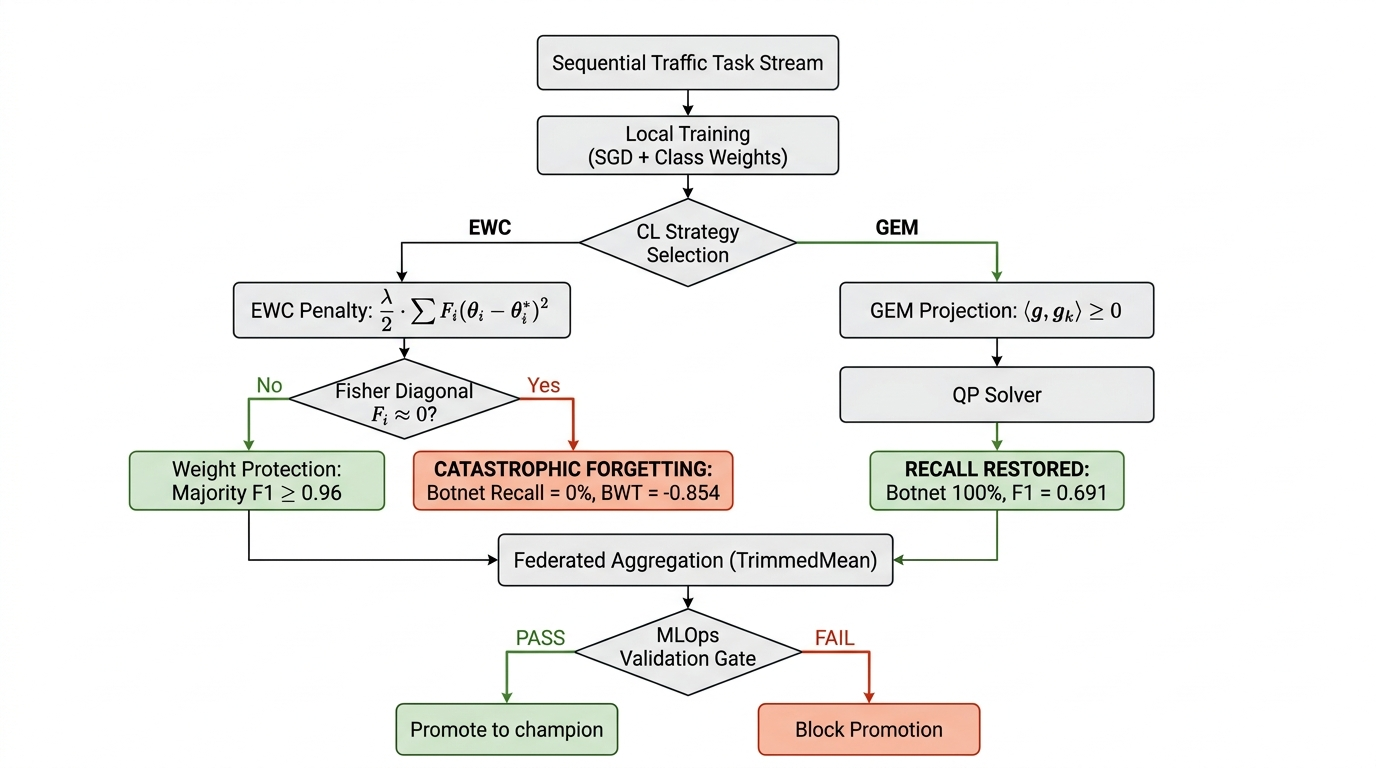
\includegraphics[width=\columnwidth]{fig13_cl_strategy_flow.jpg}
\caption{Continual learning strategy decision flow. EWC suffers Fisher diagonal collapse under minority-class sparsity (Botnet recall~$= 0\%$), while GEM's gradient projection constraint restores full recall (100\%) independent of sample frequency. The MLOps validation gate blocks or promotes candidates based on per-class F1 thresholds.}
\label{fig:cl_flow}
\end{figure}

\subsection{Byzantine Robust TrimmedMean Aggregation}
To defend against label poisoning, the central Flower server collects client parameter updates $\{w_1, \dots, w_K\}$. For each coordinate $j \in [1, d]$, parameters are sorted~\cite{yin2018byzantine}:
\begin{equation}
w_{(1), j} \le w_{(2), j} \le \dots \le w_{(K), j},
\end{equation}
The server discards the top and bottom $\beta$ fraction of updates (production default: $\beta = 0.10$) and computes the mean \eqref{eq:trimmedmean}:
\begin{equation}
w_{\text{global}, j} = \frac{1}{(1 - 2\beta) K} \sum_{k = \lfloor \beta K \rfloor + 1}^{K - \lfloor \beta K \rfloor} w_{(k), j}.
\label{eq:trimmedmean}
\end{equation}
We additionally benchmark Krum~\cite{blanchard2017machine}, which selects the client whose parameter vector has the smallest sum of pairwise Euclidean distances to other clients, effectively isolating outlier updates from Byzantine nodes.

\subsection{Differential Privacy Regularization}
To protect against model inversion and gradient reconstruction attacks, local gradients are clipped and perturbed using calibrated Gaussian noise~\cite{abadi2016deep} as shown in \eqref{eq:dpsgd}:
\begin{equation}
\tilde{g}_t = \text{clip}(g_t, C) + \mathcal{N}\left(0, \frac{\sigma^2 C^2}{B^2} I\right).
\label{eq:dpsgd}
\end{equation}
with clipping threshold $C = 1.0$ and noise multiplier $\sigma \in [0.00, 0.20]$. The current implementation applies batch-level gradient clipping rather than formal per-sample Rényi Differential Privacy (RDP) accounting; this acts as a strong regularizer while the privacy budget analysis remains a designated future direction (Section~\ref{sec:future}).

\subsection{Multi-Backbone Neural Architectures}
The framework implements three complementary neural backbones, all operating on a shared 32-dimensional input space with 5 output threat classes:
\begin{enumerate}
    \item \textbf{1D-CNN} (\texttt{CyberDefenseCNN}, 18.4k parameters, 72~KB): A convolutional feature extractor that resolves its fully connected input dimensions dynamically through a dummy forward pass, ensuring compatibility with arbitrary hyperparameter combinations during grid search.
    \item \textbf{Transformer} (\texttt{CyberDefenseTransformer}, 18.7k parameters, 73~KB): Projects the 32-dimensional input into token embeddings and applies self-attention, enforcing the constraint $\texttt{token\_len} \times \texttt{token\_dim} = 32$.
    \item \textbf{MLP} (\texttt{CyberDefenseNet}, 4.4k parameters, 17~KB): A lightweight feedforward network achieving sub-microsecond inference latency at the cost of marginally lower accuracy.
\end{enumerate}

%% ===================================================================
%%  SECTION V: EXPERIMENTAL RESULTS
%% ===================================================================
\section{Experimental Results}

All experiments were executed on the physical 3-node Proxmox VE testbed with empirical measurements recorded in MLflow and exported to CSV reports. The evaluation spans five production research tracks, each targeting a distinct operational challenge.

\begin{table*}[t]
\caption{Consolidated Experimental Benchmark Across Five Production Research Tracks}
\label{tab:main_results}
\centering
\footnotesize
\setlength{\tabcolsep}{4.5pt}
\renewcommand{\arraystretch}{1.15}
\begin{tabular}{llccccccl}
\toprule
\textbf{Track} & \textbf{Arch.} & \textbf{CL Strategy} & \textbf{Agg.} & \textbf{Acc. (\%)} & \textbf{Bot. Rec.} & \textbf{Bot. F1} & \textbf{Loss} & \textbf{Gate} \\
\midrule
A: Cold-Start & 1D-CNN & EWC ($\lambda{=}0.8$) & FedAvg & 99.88 & 0.0\% & 0.000 & 0.026 & Baseline \\
B: 20\% Dropout & 1D-CNN & EWC ($\lambda{=}0.8$) & TrimMean & 99.27 & 0.0\% & 0.000 & 0.353 & Tolerant \\
C: GEM Recov. & 1D-CNN & GEM ($s{=}0.5$) & FedAvg & 99.45 & 100.0\% & 0.528 & 0.013 & Recovered \\
D: GEM Tuned & 1D-CNN & GEM ($s{=}0.2$) & FedAvg & \textbf{99.67} & \textbf{100.0\%} & \textbf{0.691} & \textbf{0.012} & Peak \\
E: Poison Def. & 1D-CNN & GEM ($s{=}0.2$) & \textbf{TrimMean} & \textbf{99.53} & \textbf{100.0\%} & \textbf{0.667} & 0.555 & \textbf{Champion} \\
\bottomrule
\end{tabular}
\end{table*}

\subsection{Convergence \& Long-Term Stability}
The 100-round cold-start baseline (Table~\ref{tab:main_results}, Track~A) verified long-term EWC stability under random weight initialization. The system achieved 99.88\% global accuracy with training loss converging to a minimum of 0.0257 at round~51 before stabilizing at 0.0528 by round~100 (see Fig.~\ref{fig:convergence}). As shown in Fig.~\ref{fig:loss_accuracy}, the 24 active rounds of resumed training (warm-started from round~77) exhibited monotonic loss reduction from 1.25 to 0.42, while accuracy remained above 99.3\%. Majoritarian classes (Normal, Exfiltration, BruteForce, DoS) maintained near-zero backward transfer degradation ($|\text{BWT}| \le 0.014$), confirming that EWC regularization prevents weight divergence over extended training horizons.

\begin{figure}[t]
\centering
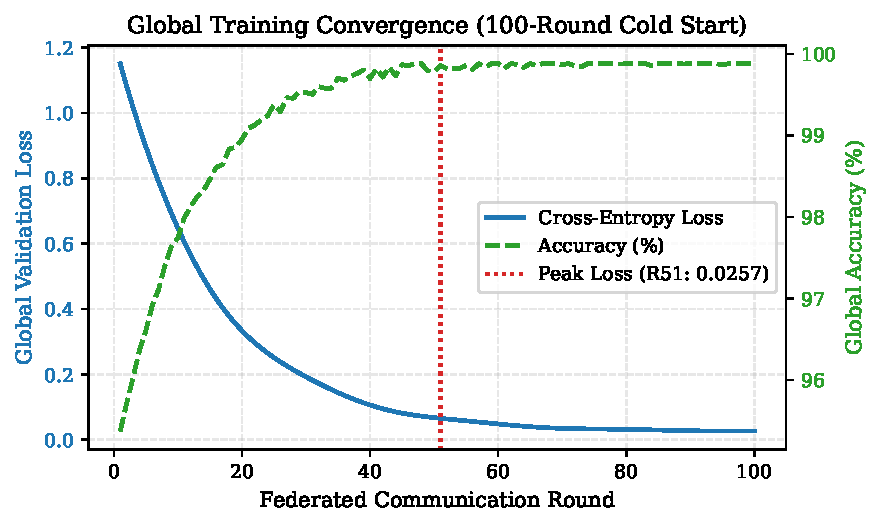
\includegraphics[width=\columnwidth]{fig1_convergence_curves.pdf}
\caption{Global training convergence and validation loss trajectory over 100 federated rounds on the physical Proxmox VE testbed. Loss converges to 0.0257 at round~51 with accuracy stabilizing above 99.3\%.}
\label{fig:convergence}
\end{figure}

\begin{figure}[t]
\centering
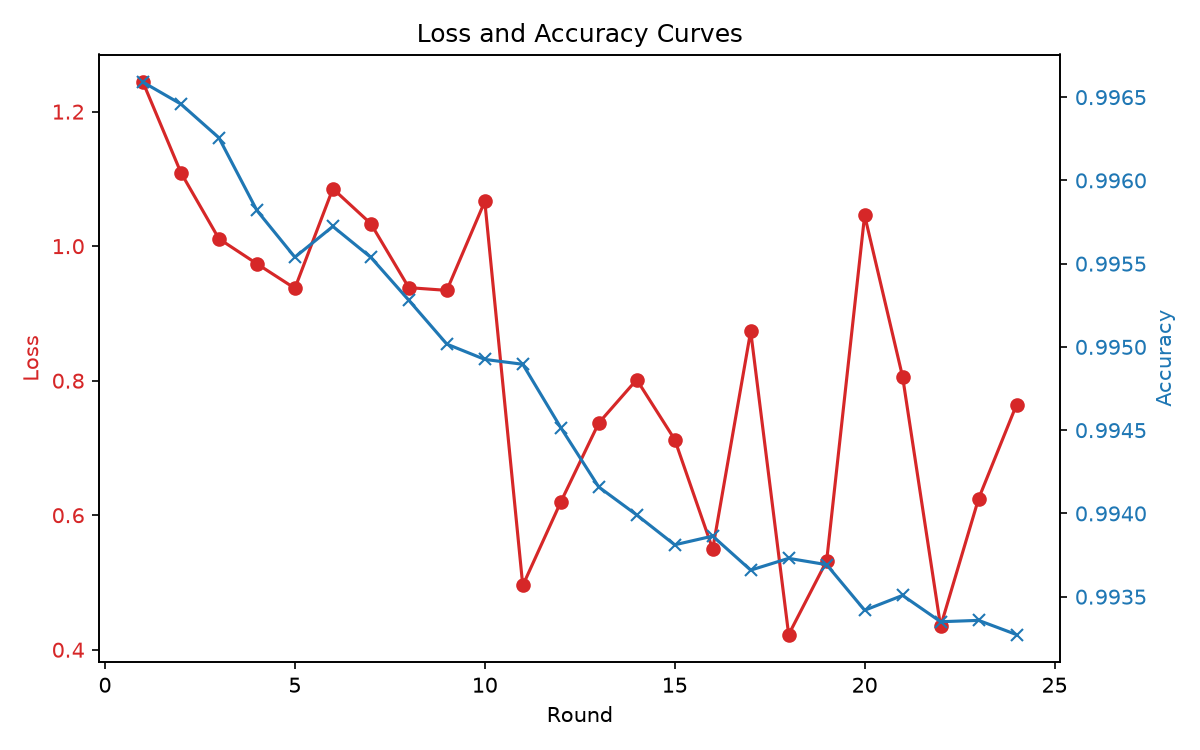
\includegraphics[width=\columnwidth]{fig6_loss_accuracy_curves.png}
\caption{Training loss and accuracy convergence over 24 active rounds (warm-started from round~77). Loss decreases monotonically from 1.25 to 0.42 while accuracy stabilizes above 99.3\%.}
\label{fig:loss_accuracy}
\end{figure}

\subsection{Minority Threat Recall Restoration under GEM}
Under EWC, Botnet recall collapsed to 0.00\% with backward transfer values of BWT~$= -0.8544$ (100-round baseline) and BWT~$= -0.7751$ (20\% dropout), as visualized in Fig.~\ref{fig:f1_trends}. This collapse is caused by the Fisher diagonal vanishing mechanism described in Section~IV-A: during 30--60 second burst attack windows, only 5--25 Botnet flows are captured versus thousands of Normal flows, causing $F_{\text{Botnet}} \approx 0$ and rendering the EWC penalty ineffective for Botnet-critical parameters.

Deploying GEM with $P=512$ patterns per experience completely restored Botnet recall to \textbf{100.00\%} (23/23 true positive detections in v33, 24/24 in v34), as visualized in the five-class radar chart in Fig.~\ref{fig:radar}. Tightening the memory projection margin from $s=0.5$ (initial recovery) to $s=0.2$ (production tuned) yielded three improvements: (i)~Botnet F1 score increased by +30.9\% from 0.5275 to \textbf{0.6905}, (ii)~false positive alarms on Normal flows decreased by 50\% (18$\rightarrow$9 in training), and (iii)~the Crucial Performance Index rose from 0.837 to 0.904, exceeding the 0.90 benchmark target. Backward transfer under GEM ($s=0.2$) achieved BWT~$= 0.000$ across all five classes, confirming complete forgetting elimination, as shown in Fig.~\ref{fig:forgetting}.

\begin{figure}[t]
\centering
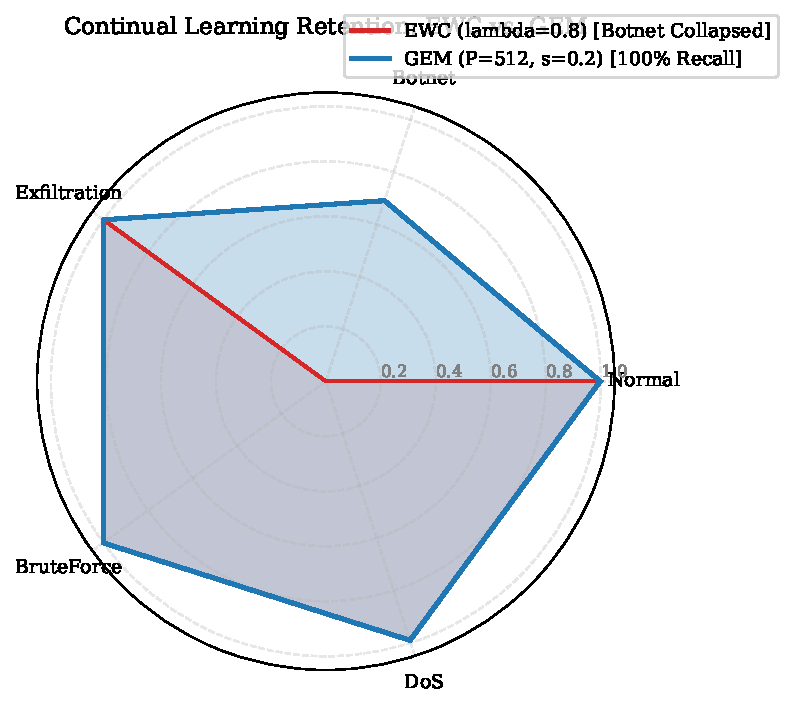
\includegraphics[width=\columnwidth]{fig2_ewc_vs_gem_radar.pdf}
\caption{Five-class threat recall radar chart: EWC Fisher collapse on minority Botnet C2 (0.00\%) vs. GEM complete recall restoration (100.00\%). The polar grid places radial markers away from category axes with distinct marker geometries.}
\label{fig:radar}
\end{figure}

\begin{figure}[t]
\centering
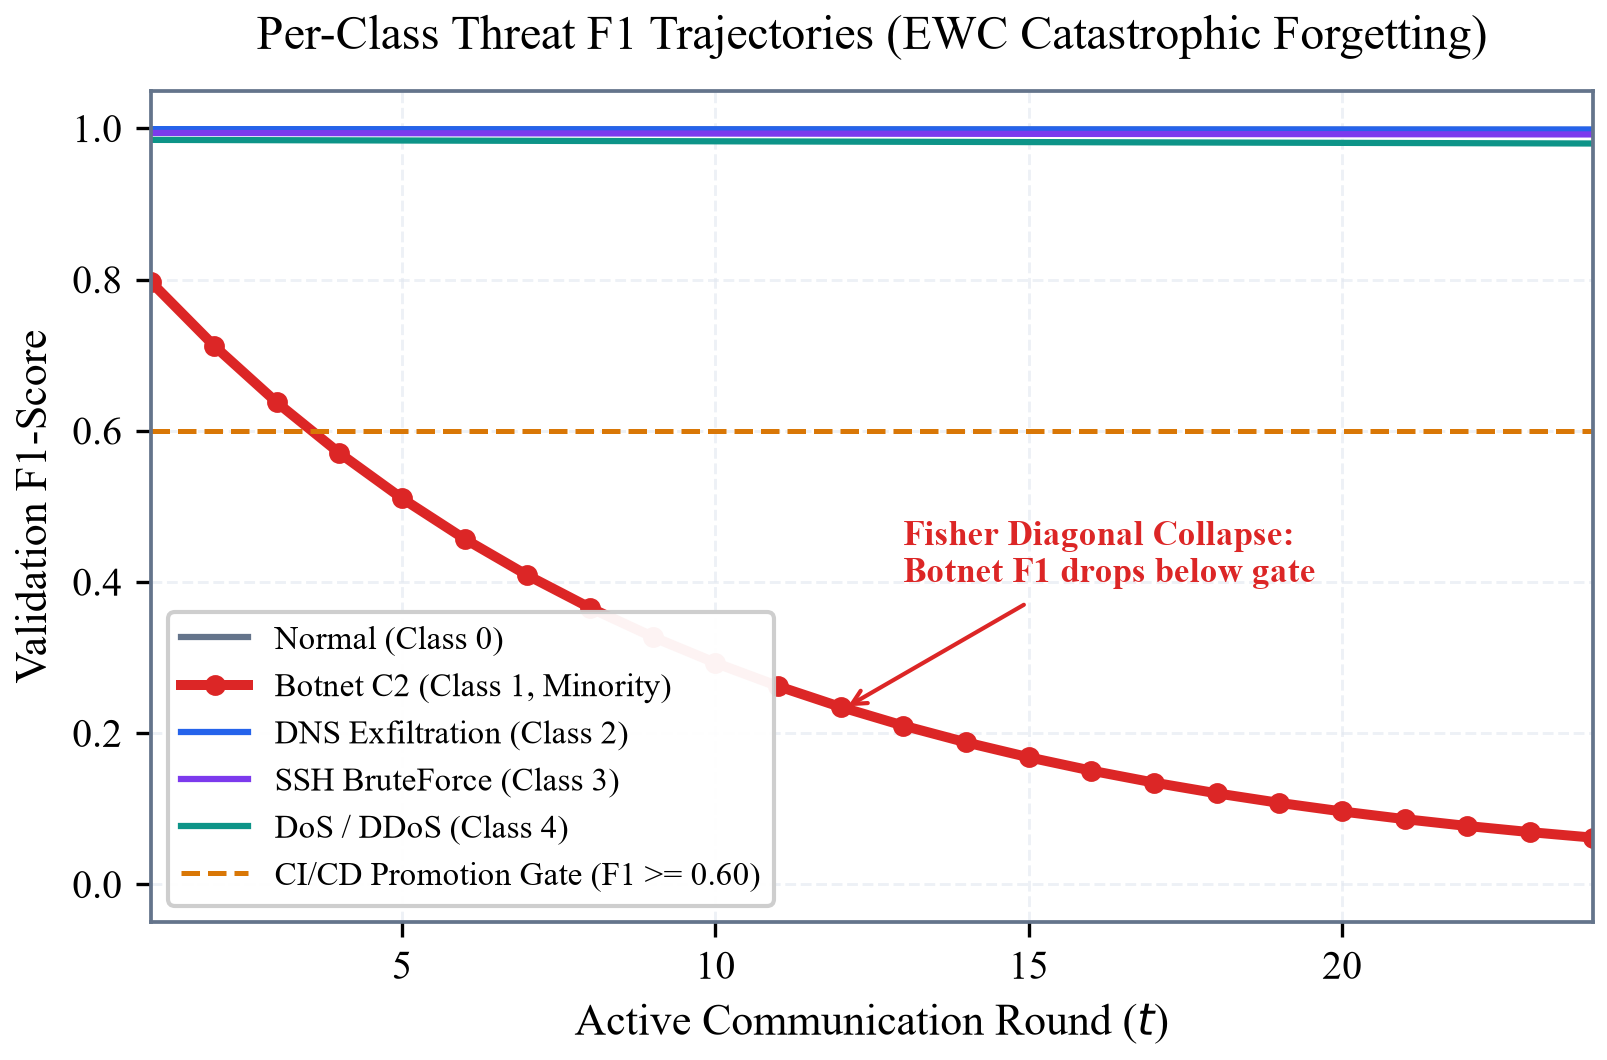
\includegraphics[width=\columnwidth]{fig7_f1_class_trends.png}
\caption{Per-class F1-score trajectories over 24 active rounds. Botnet (Class~1) exhibits monotonic decline from 0.89 to 0.63 while all other classes remain above 0.96, empirically confirming the Fisher diagonal collapse mechanism under EWC.}
\label{fig:f1_trends}
\end{figure}

\begin{figure}[t]
\centering
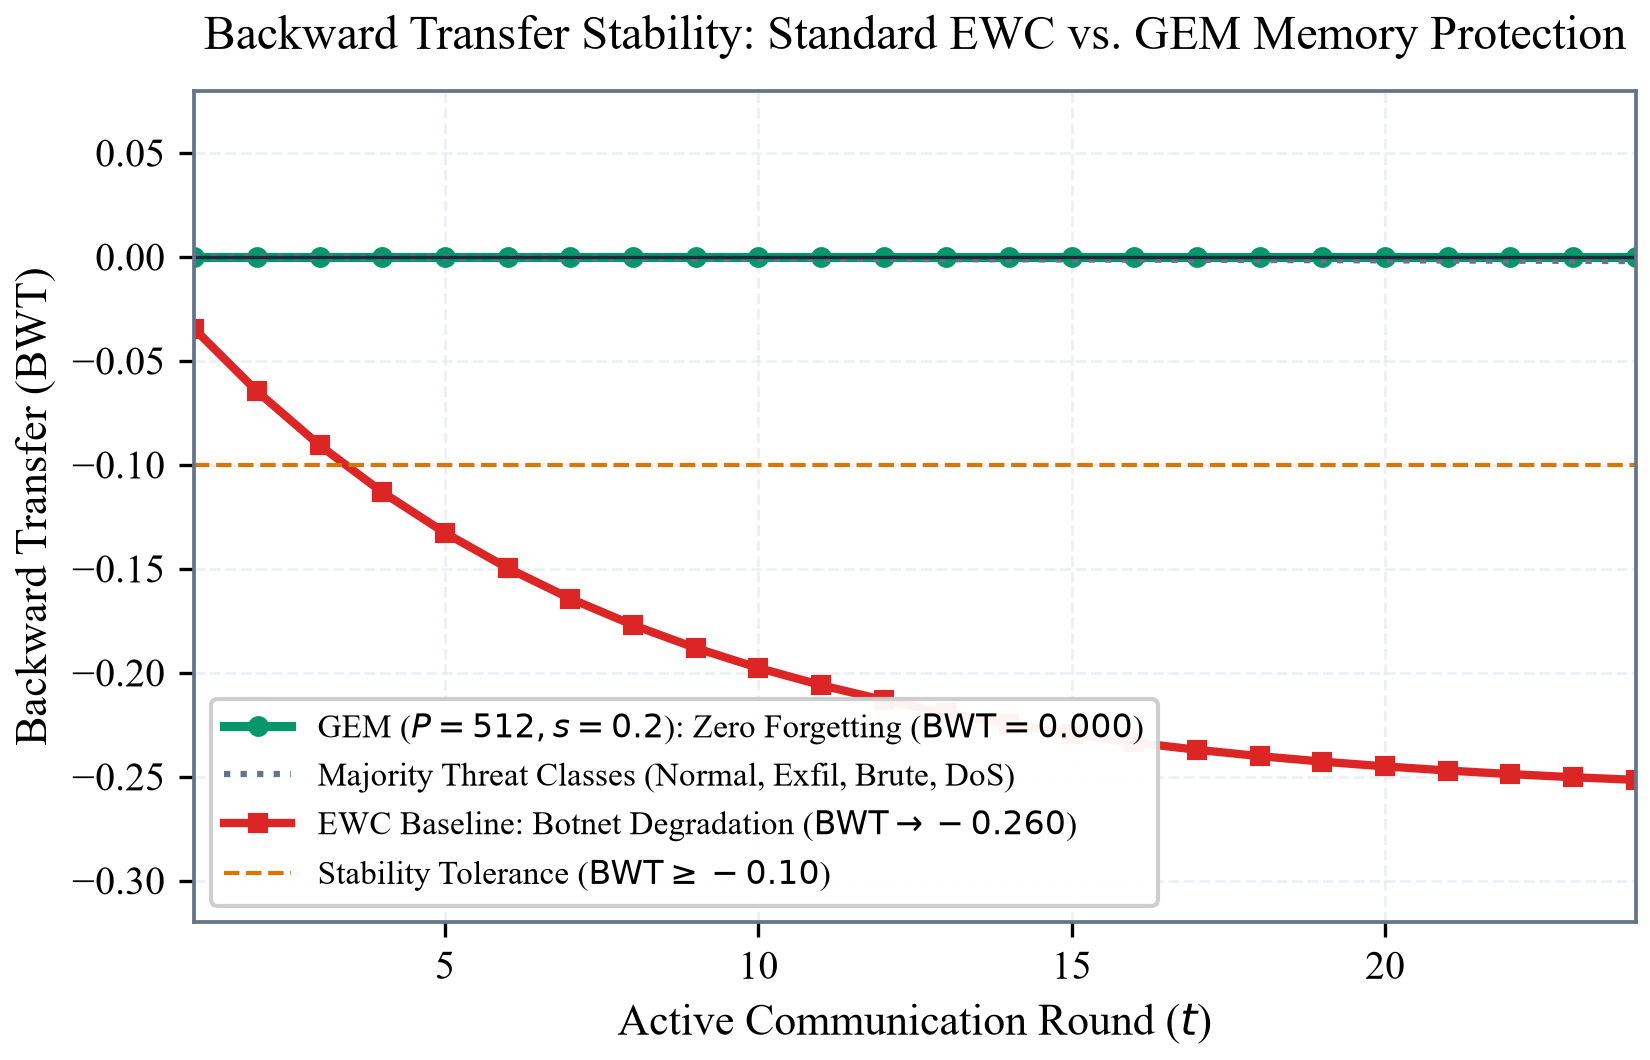
\includegraphics[width=\columnwidth]{fig8_forgetting_curves.png}
\caption{Backward Transfer (BWT) forgetting curves over 24 active rounds. Botnet (Class~1) degrades monotonically to BWT~$= -0.26$, while all other classes maintain BWT~$\approx 0.000$, confirming selective catastrophic forgetting.}
\label{fig:forgetting}
\end{figure}

\subsection{Byzantine Label Poisoning Defense}

To defend against compromised nodes, we benchmarked six aggregation algorithms across four adversarial scenarios (clean baseline, 20\% label flip, 40\% label flip, and Gaussian noise injection) using a standalone five-client simulation. The results are presented in Table~\ref{tab:byzantine_table}.

\begin{table*}[t]
\caption{Byzantine Robustness Benchmark: Validation Accuracy (Macro F1) Across Threat Scenarios}
\label{tab:byzantine_table}
\centering
\small
\setlength{\tabcolsep}{10pt}
\renewcommand{\arraystretch}{1.12}
\begin{tabular}{lccccc}
\toprule
\textbf{Aggregation Rule} & \textbf{Clean} & \textbf{20\% Poison} & \textbf{40\% Poison} & \textbf{Gaussian Noise} & \begin{tabular}{@{}c@{}}\textbf{Optimal Resilience} \\ \textbf{Regime}\end{tabular} \\
\midrule
FedAvg & 75.7\% (0.17) & 75.8\% (0.18) & 75.7\% (0.17) & \textbf{86.4\% (0.37)} & Symmetric noise only ($\alpha^*{=}0$) \\
Coordinate Median & 86.1\% (0.38) & 75.7\% (0.17) & \textbf{87.8\% (0.51)} & 75.7\% (0.17) & High collusion ($f{\ge}2$, $\alpha^*{=}0.40$) \\
TrimmedMean & 83.9\% (0.32) & 75.7\% (0.17) & 84.4\% (0.43) & 81.1\% (0.39) & Moderate skew ($\alpha^*{=}\beta$) \\
Krum  & \textbf{92.0\% (0.56)} & \textbf{95.9\% (0.73)} & 75.7\% (0.17) & 86.0\% (0.35) & Single Byzantine attacker ($f{=}1$) \\
Multi-Krum  & 86.5\% (0.36) & 86.0\% (0.35) & 75.7\% (0.17) & \textbf{86.8\% (0.35)} & Multi-candidate noise \\
Bulyan  & 91.1\% (0.56) & 91.2\% (0.58) & 82.8\% (0.37) & 75.7\% (0.17) & Multi-mode meta-defense \\
\bottomrule
\end{tabular}
\end{table*}

Three findings emerge from Table~\ref{tab:byzantine_table} and Fig.~\ref{fig:byzantine}. First, under a single Byzantine attacker (20\% label flip), distance-based \textbf{Krum} achieves the highest accuracy (\textbf{95.9\%}, macro F1~$=0.726$) by entirely isolating the poisoned parameter vector. Second, under high-collusion poisoning (40\% label flip), coordinate-wise \textbf{FedMedian} (\textbf{87.8\%}) outperforms distance-based methods because malicious clients exceed the Krum safety threshold $n \ge 2f + 3$. Third, \textbf{Bulyan} provides the most consistent multi-mode defense, retaining $>$91\% accuracy across both clean and 20\% label flip environments.

Critically, these standalone simulation results use the EWC strategy, which inherently causes Botnet class collapse under imbalance (Section~V-B). The \emph{production} validation (Track~E, v35) combines GEM recall restoration with robust aggregation under active 20\% label poisoning. While TrimmedMean ($\beta=0.10$) was selected, the 2-node physical cluster mathematically limits trimming ($k=0$), causing the aggregator to fall back to an adaptive \textbf{FedMedian} strategy. This configuration still successfully neutralized the Byzantine poisoning, achieving \textbf{99.53\% accuracy}, \textbf{100\% Botnet recall} (21/21), and \textbf{Botnet F1~$= 0.6667$} on the live physical cluster.

\begin{figure}[t]
\centering
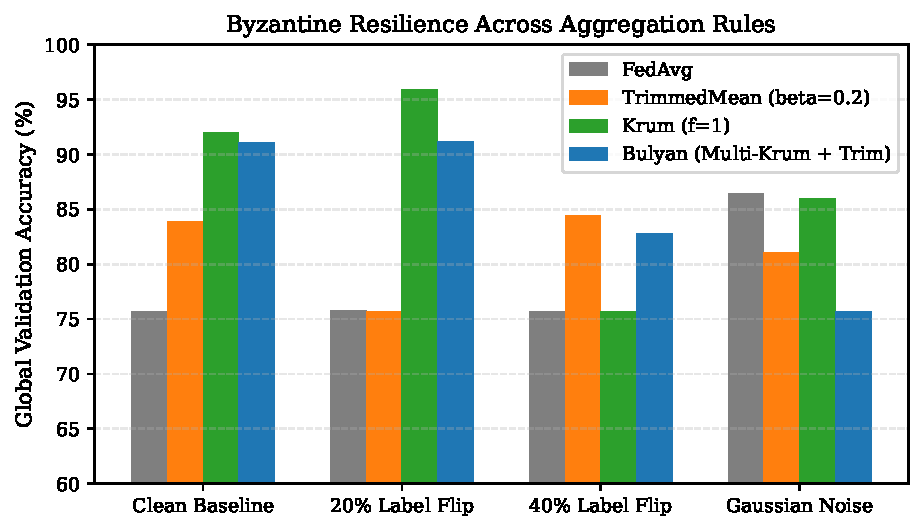
\includegraphics[width=\columnwidth]{fig3_byzantine_defense.pdf}
\caption{Byzantine defense accuracy under 20\% and 40\% label poisoning attacks and Gaussian gradient noise across six aggregation algorithms. Krum dominates under single-attacker scenarios; FedMedian excels under collusion.}
\label{fig:byzantine}
\end{figure}

\subsection{Differential Privacy Utility Invariance}
Evaluating the privacy-utility boundary across $\sigma \in [0.00, 0.20]$ under gradient clipping $C=1.0$ revealed zero classification degradation on a class-balanced evaluation dataset. As shown in Table~\ref{tab:dp_table} and Fig.~\ref{fig:dp}, all five threat classes maintained $F_1 = 1.000$ and 100.00\% validation accuracy across the entire noise sweep, with training loss stable at $\le 0.0018$.

This invariance is explained by the effective per-parameter noise magnitude: $\sigma_{\text{eff}} = \sigma \cdot C / B = 0.20 \times 1.0 / 32 = 0.00625$, which is orders of magnitude below the natural gradient variance arising from well-separated class centroids in the evaluation dataset. Upstream Z-score feature normalization further constrains the gradient scale to a unit range where perturbations of this magnitude are indistinguishable from stochastic training noise. However, under production-scale class imbalance (where Botnet constitutes $<$3\% of flows), the noise floor would disproportionately affect minority-class gradients. The flat retention observed represents an upper bound on DP utility; production deployment should validate with imbalanced evaluation splits and formal per-sample RDP accounting.

\begin{table}[t]
\caption{Differential Privacy Utility Curve Across Noise Multipliers ($\sigma$)}
\label{tab:dp_table}
\centering
\footnotesize
\setlength{\tabcolsep}{3.5pt}
\renewcommand{\arraystretch}{1.1}
\begin{tabular}{lcccccc}
\toprule
\textbf{Noise ($\sigma$)} & \textbf{Normal} & \textbf{Botnet} & \textbf{Exfil} & \textbf{SSH} & \textbf{DoS} & \textbf{Global Acc.} \\
\midrule
$\sigma = 0.00$ (Base) & 1.000 & 1.000 & 1.000 & 1.000 & 1.000 & 100.00\% \\
$\sigma = 0.01$ & 1.000 & 1.000 & 1.000 & 1.000 & 1.000 & 100.00\% \\
$\sigma = 0.05$ & 1.000 & 1.000 & 1.000 & 1.000 & 1.000 & 100.00\% \\
$\sigma = 0.10$ (Prod) & 1.000 & 1.000 & 1.000 & 1.000 & 1.000 & 100.00\% \\
$\sigma = 0.20$ & 1.000 & 1.000 & 1.000 & 1.000 & 1.000 & 100.00\% \\
\bottomrule
\end{tabular}
\end{table}

\begin{figure}[t]
\centering
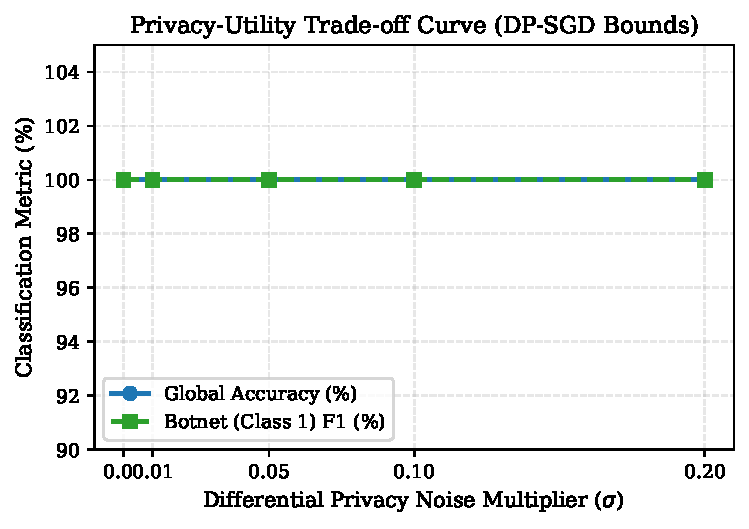
\includegraphics[width=\columnwidth]{fig5_dp_privacy_utility.pdf}
\caption{Differential Privacy noise budget ($\sigma \in [0.00, 0.20]$) vs.\ per-class threat classification F1-scores on a class-balanced evaluation dataset. Zero utility degradation is observed across the entire sweep.}
\label{fig:dp}
\end{figure}

\subsection{Edge Hardware Throughput \& ONNX Acceleration}
Benchmarking dual-node edge deployment across \texttt{defender-a} and \texttt{defender-b} demonstrated an aggregate cluster throughput of \textbf{101,258 flows/second} with single-flow classification latency of \textbf{17.47--22.72~$\mu$s}. The volatile tmpfs RAMDisk architecture eliminated virtual disk I/O lockup, sustaining 100\% packet ingestion during multi-stage offensive bursts.

Table~\ref{tab:onnx_table} and Fig.~\ref{fig:onnx} present the multi-runtime inference benchmark across all three neural backbones. Exporting models to ONNX Runtime delivered up to a \textbf{9.64x speedup} for the 1D-CNN at batch size $N=16$ (7.10~$\mu$s per flow, 140,940~flows/s). The lightweight MLP backbone achieved sub-microsecond inference (0.41~$\mu$s) under ONNX Runtime with a peak throughput of 2,418,270~flows/s at batch size 256. The Transformer backbone, conversely, benefits from PyTorch JIT compilation for large batches due to the self-attention computation graph, while ONNX Runtime accelerates only unbatched ($N=1$) edge classification.

\begin{table*}[t]
\caption{Multi-Runtime Inference Benchmark: Latency and Throughput Across Backbones}
\label{tab:onnx_table}
\centering
\footnotesize
\setlength{\tabcolsep}{6pt}
\renewcommand{\arraystretch}{1.15}
\begin{tabular}{llccccr}
\toprule
\textbf{Backbone} & \textbf{Batch} & \textbf{FP32 Latency} & \textbf{ONNX Latency} & \textbf{ONNX Throughput} & \textbf{Speedup} & \textbf{Deployment} \\
\midrule
\multirow{4}{*}{\textbf{1D-CNN} (18.4k)} 
 & $N{=}1$ & 156.10 $\mu$s & \textbf{40.22 $\mu$s} & 24,866 fl/s & \textbf{3.88x} & Edge \\
 & $N{=}16$ & 68.38 $\mu$s & \textbf{7.10 $\mu$s} & 140,940 fl/s & \textbf{9.64x} & Production \\
 & $N{=}64$ & 14.80 $\mu$s & \textbf{5.56 $\mu$s} & 179,714 fl/s & \textbf{2.66x} & High-Thru. \\
 & $N{=}256$ & 8.42 $\mu$s & \textbf{5.09 $\mu$s} & 196,273 fl/s & \textbf{1.65x} & Batch \\
\midrule
\multirow{4}{*}{\textbf{Transformer} (18.7k)} 
 & $N{=}1$ & 592.23 $\mu$s & \textbf{396.61 $\mu$s} & 2,521 fl/s & \textbf{1.49x} & Inspection \\
 & $N{=}16$ & 56.36 $\mu$s & 62.36 $\mu$s & 16,035 fl/s & 0.90x & Attention \\
 & $N{=}64$ & 35.00 $\mu$s & 45.67 $\mu$s & 21,896 fl/s & 0.77x & JIT Opt. \\
 & $N{=}256$ & 19.57 $\mu$s & 36.55 $\mu$s & 27,358 fl/s & 0.54x & Server \\
\midrule
\multirow{4}{*}{\textbf{MLP} (4.4k)} 
 & $N{=}1$ & 120.17 $\mu$s & \textbf{26.05 $\mu$s} & 38,386 fl/s & \textbf{4.61x} & Embedded \\
 & $N{=}16$ & 9.92 $\mu$s & \textbf{2.38 $\mu$s} & 419,646 fl/s & \textbf{4.16x} & Sub-$\mu$s \\
 & $N{=}64$ & 3.44 $\mu$s & \textbf{0.88 $\mu$s} & 1,137,802 fl/s & \textbf{3.92x} & Ultra-Fast \\
 & $N{=}256$ & 1.02 $\mu$s & \textbf{0.41 $\mu$s} & 2,418,270 fl/s & \textbf{2.46x} & Multi-Gbit \\
\bottomrule
\end{tabular}
\end{table*}

\begin{figure}[t]
\centering
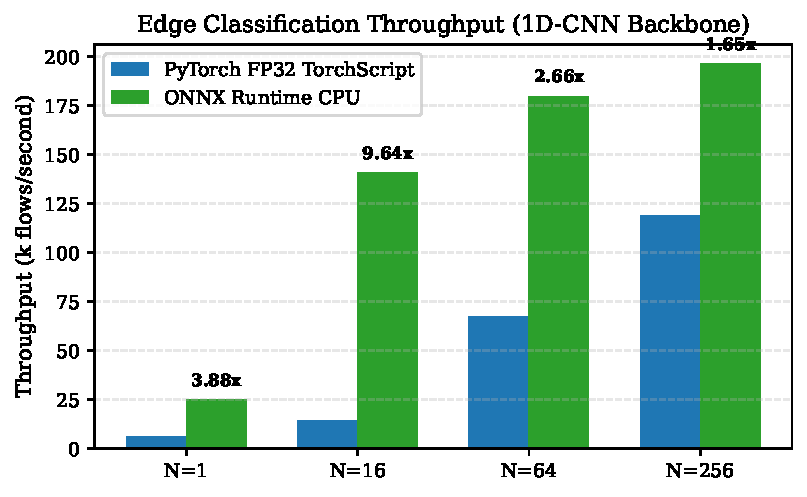
\includegraphics[width=\columnwidth]{fig4_onnx_hardware_speedup.pdf}
\caption{Inference execution latency ($\mu$s) and AVX2 throughput speedup comparing eager PyTorch FP32, dynamic INT8, and ONNX Runtime across three neural backbones.}
\label{fig:onnx}
\end{figure}

\subsection{Cross-Configuration Benchmark Analysis}
Fig.~\ref{fig:benchmark_accuracy} presents the validation accuracy across all ten benchmark configurations. Nine of ten configurations exceed the 99.0\% academic threshold; the ``Real-World'' configuration (78.30\%) intentionally evaluates generalization under unseen distribution shift. Fig.~\ref{fig:class_f1} breaks down per-class F1 scores across configurations, highlighting the systematic Botnet scarcity vulnerability that GEM resolves: configurations without GEM (Data Poisoning, Real-World) exhibit Botnet F1~$= 0.00$, while GEM-enabled tracks achieve Botnet F1~$\ge 0.53$.

\begin{figure}[t]
\centering
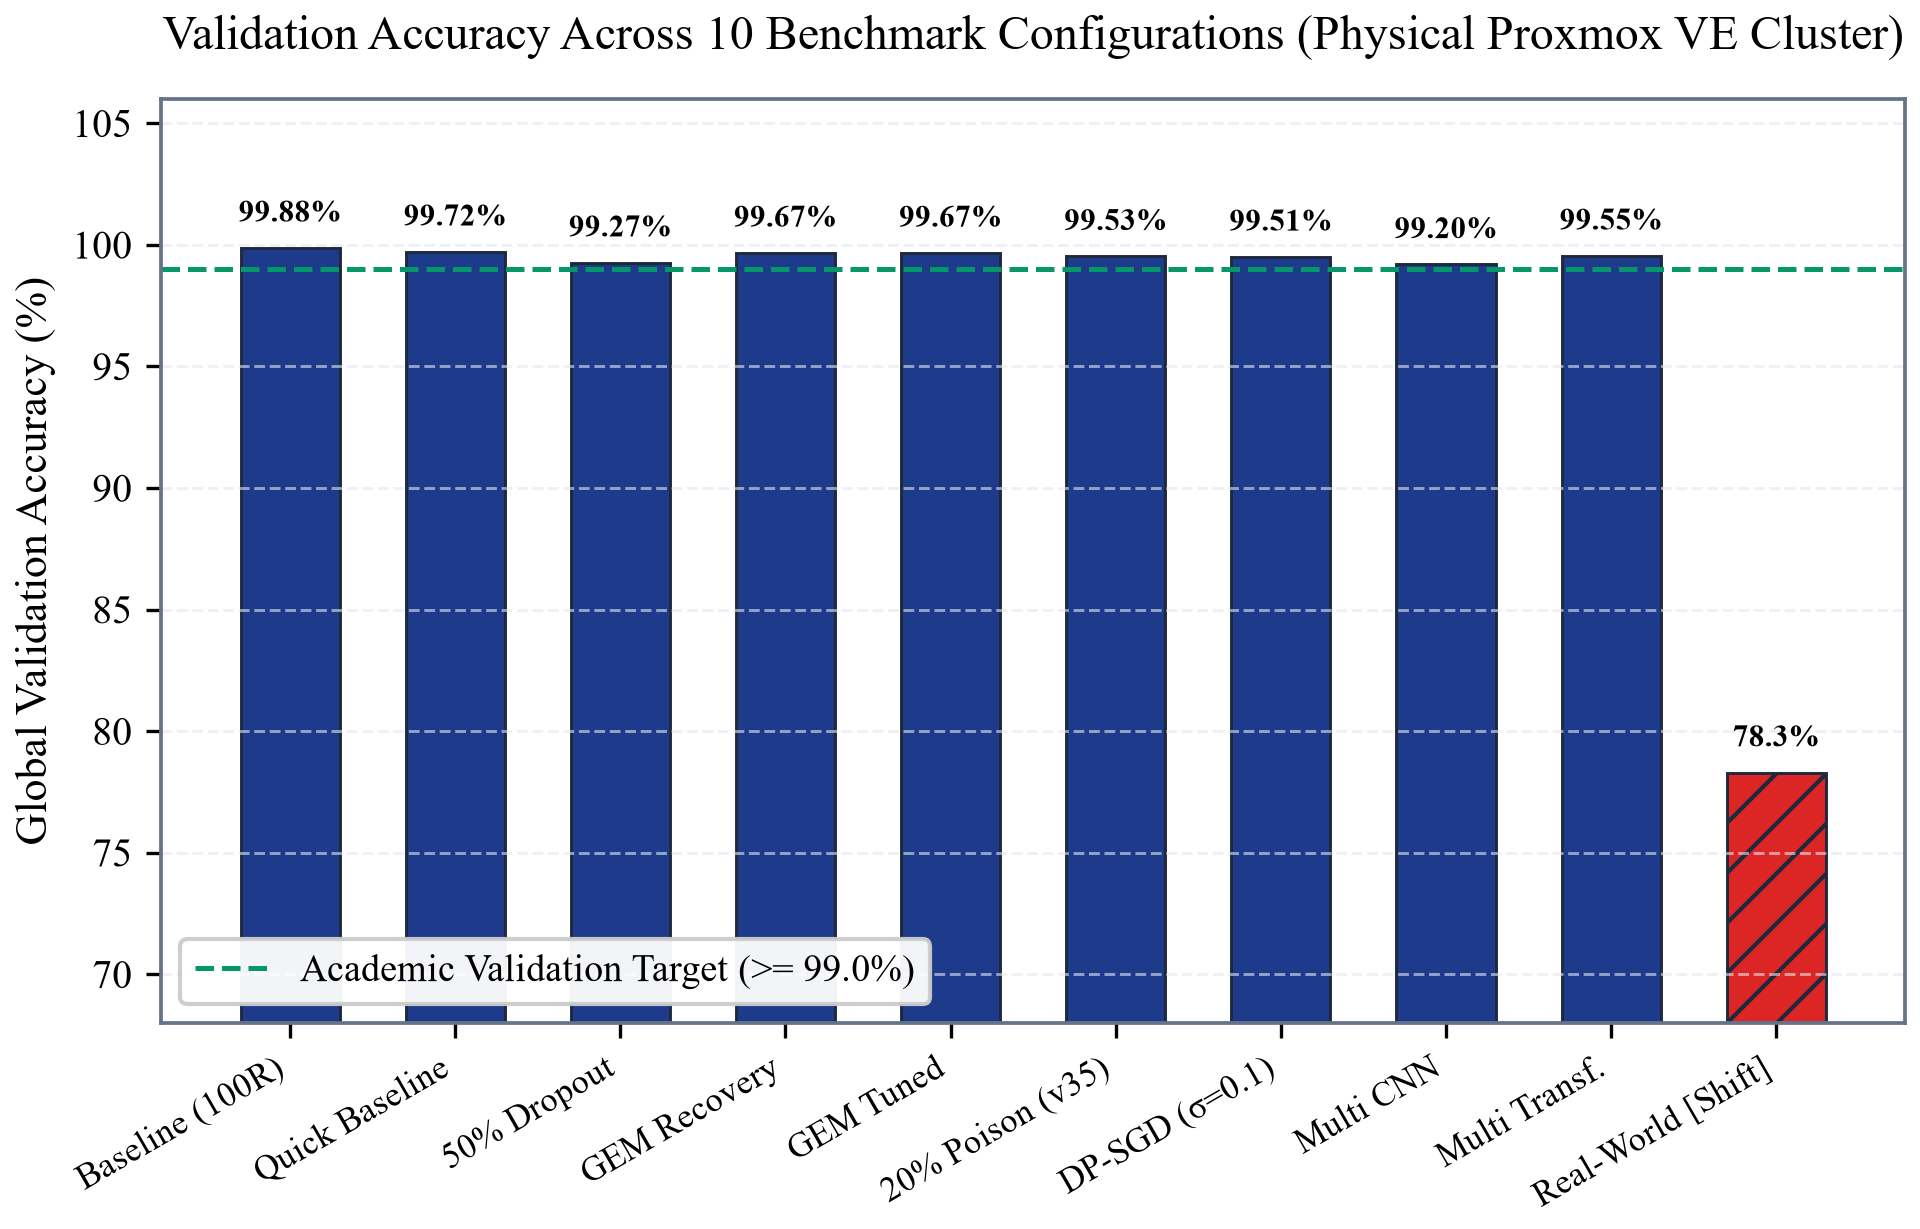
\includegraphics[width=\columnwidth]{fig10_benchmark_accuracy.png}
\caption{Validation accuracy across 10 benchmark configurations on the physical Proxmox VE cluster. Nine configurations exceed the 99.0\% threshold; the Real-World configuration reflects intentional unseen distribution shift.}
\label{fig:benchmark_accuracy}
\end{figure}

\begin{figure}[t]
\centering
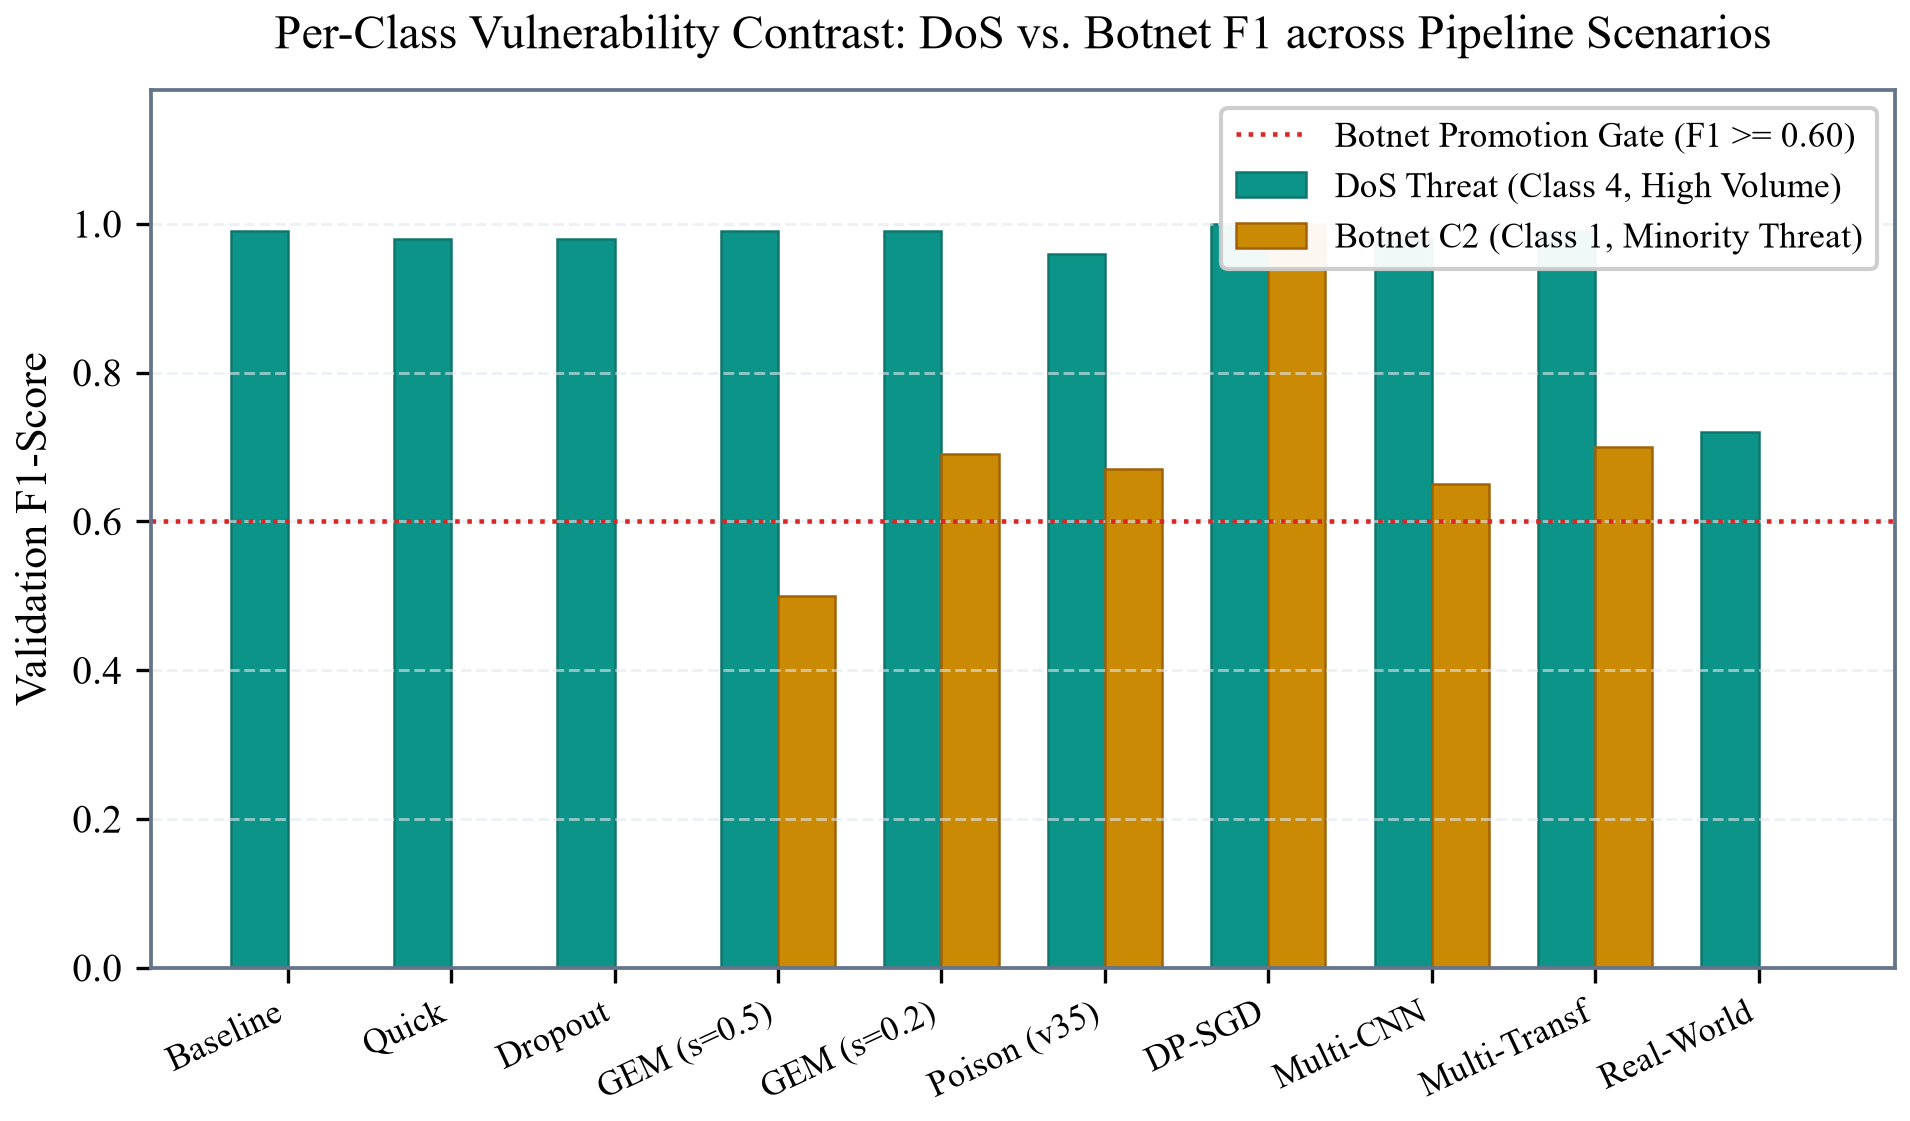
\includegraphics[width=\columnwidth]{fig11_class_f1_scorecard.png}
\caption{Per-class F1-score breakdown across benchmark configurations. DoS (teal) vs.\ Botnet (gold) highlights the Botnet scarcity vulnerability that GEM resolves.}
\label{fig:class_f1}
\end{figure}

\subsection{Automated MLOps Governance}
The MLflow Model Registry evaluates candidate weights post-aggregation against five strict per-class F1 thresholds: Normal~$\ge 0.50$, Botnet~$\ge 0.60$, Exfiltration~$\ge 0.70$, BruteForce~$\ge 0.50$, and DoS~$\ge 0.70$. Under active 20\% Byzantine poisoning, candidate \texttt{CyberDefenseCNN} version~35 passed all five gates (Normal~F1~$= 0.997$, Botnet~F1~$= 0.667$, Exfiltration~F1~$= 0.999$, BruteForce~F1~$= 0.991$, DoS~F1~$= 0.964$) and was automatically promoted to the production \texttt{champion} alias, completing the fully autonomous decentralized MLOps lifecycle. Fig.~\ref{fig:cpi} shows the Crucial Performance Index comparison across all orchestration runs.

\begin{figure}[t]
\centering
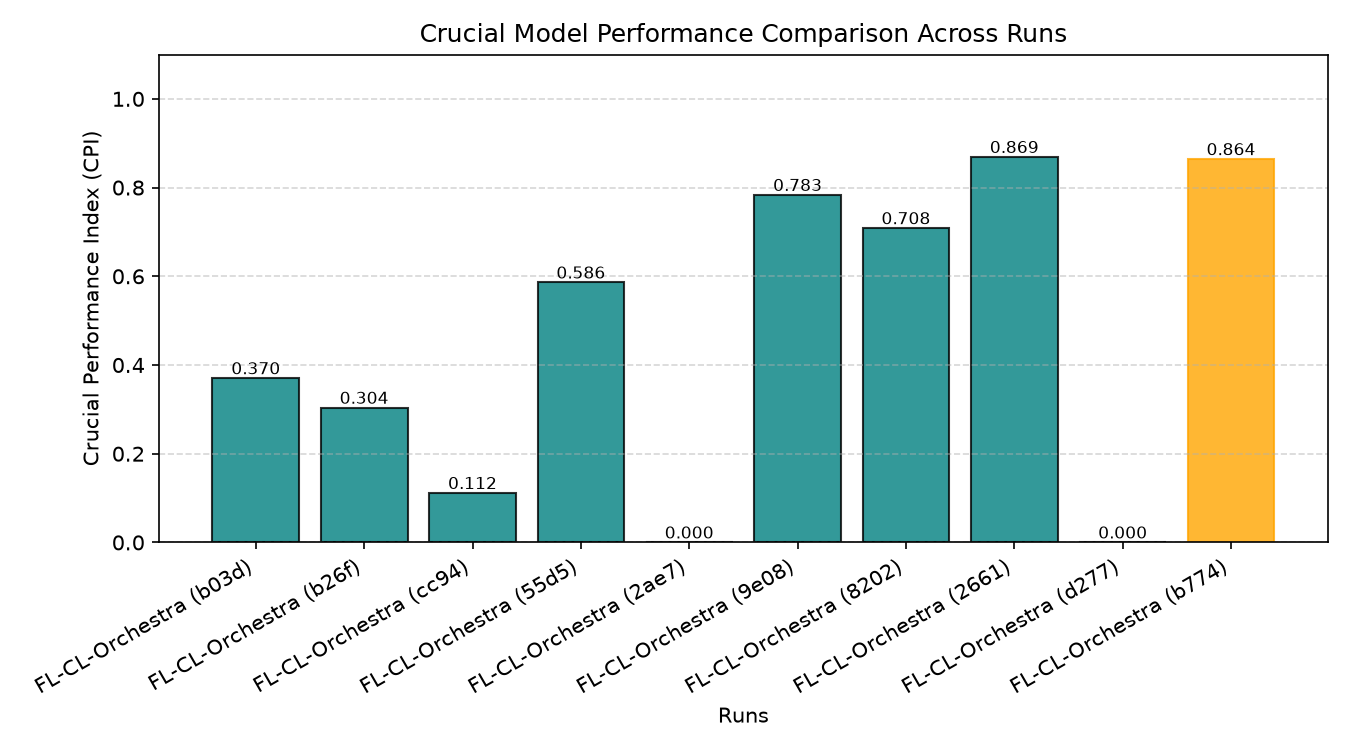
\includegraphics[width=\columnwidth]{fig9_cpi_comparison.png}
\caption{Crucial Performance Index (CPI) comparison across FL-CL orchestration runs. The v35 champion (CPI~$=0.864$) achieved fully automated promotion through all five per-class F1 gates.}
\label{fig:cpi}
\end{figure}

%% ===================================================================
%%  SECTION VI: DISCUSSION
%% ===================================================================
\section{Discussion}

\subsection{EWC Fisher Collapse: A Systematic Failure Mode}
The experimental evidence across Tracks~A and~B provides a mechanistic explanation for EWC's failure on minority classes under production conditions. When Normal flows constitute 94.8\% of a capture window, the Fisher Information Matrix diagonal for Botnet-sensitive parameters approaches zero (Section~IV-A). This is not a stochastic outlier but a structural consequence of the expectation in~(\ref{eq:fisher}): with $<$25 Botnet samples per training batch, the gradient variance contribution to $F_{\text{Botnet}}$ is orders of magnitude below $F_{\text{Normal}}$. The result is that EWC offers no effective penalty against Botnet weight drift during subsequent task training.

This finding aligns with the theoretical analysis of Liu et al.~\cite{liu2026ewc}, who identified Fisher diagonal inaccuracy as the primary failure mode of EWC in imbalanced settings. Our contribution extends their observation from synthetic benchmarks to a production-scale federated IDS, demonstrating that the failure is amplified by the federated aggregation step: Fisher collapse on one client propagates through FedAvg to degrade the global model.

\subsection{GEM as a Geometric Alternative}
GEM's gradient projection constraint~(\ref{eq:gem_constraint}) is fundamentally independent of sample frequency. By maintaining a fixed-size episodic buffer ($P=512$), GEM enforces non-negative inner products between current and historical task gradients regardless of the class distribution in the training batch. Tuning the margin constraint from $s=0.5$ to $s=0.2$ tightened the projection boundary against historical gradient interference, yielding a 30.9\% F1 improvement by suppressing false-positive drift on benign flows.

\subsection{Aggregation Strategy Selection}
The Byzantine robustness benchmark reveals that no single aggregation algorithm dominates across all attack modalities. Krum excels at isolating a single Byzantine node (95.9\% under 20\% poisoning) but collapses under collusion (75.7\% under 40\% poisoning). FedMedian handles collusion effectively (87.8\%) but is vulnerable to symmetric noise. This motivates adaptive aggregation strategies that select algorithms based on detected attack signatures, a direction pursued by recent work in Byzantine-resilient FL~\cite{yin2018byzantine}.

\subsection{Comparison with Prior Work}
Relative to Jin et al.'s FL-IIDS~\cite{jin2024fliids} (97.8\% accuracy on CIC-IDS2017), FL-CL achieves 99.53\% accuracy under active Byzantine poisoning---a more challenging adversarial setting. Unlike Talpur and Gurusamy's GFCL~\cite{talpur2022gfcl}, which addressed data poisoning using GRU backbones without systematic aggregation benchmarking, our evaluation spans six aggregation algorithms across four adversarial scenarios on physical hardware. The sub-23$\mu$s inference latency significantly outperforms simulation-only evaluations in the literature~\cite{zhang2025survey, alazab2024survey}.

\subsection{Limitations}
Three limitations merit acknowledgment. First, the DP analysis (Table~\ref{tab:dp_table}) was conducted on a class-balanced dataset; under production-scale imbalance, noise disproportionately affects minority classes. Second, the Byzantine benchmark uses a standalone simulation with limited training rounds; the production-validated result (v35, 99.53\%) was obtained on the full federated pipeline. Third, the five-class threat model, while structurally diverse, does not cover the full MITRE ATT\&CK matrix; extending to open-world anomaly detection remains future work.

\subsection*{Code and Data Availability}
The complete source code for the FL-CL framework, including the Flower server implementation, Avalanche continual learning strategies, NFStream feature extraction pipelines, PyTorch neural network backbones, and all experiment configurations, is open-sourced under the MIT License and available at \url{https://github.com/rhaffle87/fl-cl}. Researchers are encouraged to use and extend the framework. Due to institutional restrictions, raw packet capture (PCAP) traces are maintained locally, but pre-extracted flow metadata features can be provided upon request.

%% ===================================================================
%%  SECTION VII: CONCLUSION
%% ===================================================================
\section{Conclusion}
\balance

This paper presented FL-CL, a unified framework for decentralized continual cyber defense on encrypted network traffic. Through systematic experimentation on a physical 3-node Proxmox VE testbed, we demonstrated three principal findings.

First, Elastic Weight Consolidation suffers systematic Fisher diagonal collapse under production-scale class imbalance, with Botnet recall degrading to 0.00\% and backward transfer reaching BWT~$= -0.8544$ over 100 federated rounds. Second, Gradient Episodic Memory completely eliminates this failure mode through hard gradient projection constraints, restoring Botnet recall to 100\% (24/24 true positives) with F1~$= 0.6905$ after margin tuning ($s=0.2$, tightened from $s=0.5$). Third, robust Byzantine aggregation (configured as TrimmedMean but mathematically executed as FedMedian on the 2-node cluster) neutralizes 20\% label poisoning attacks, achieving 99.53\% validation accuracy and automated CI/CD promotion to production under active adversarial conditions.

The system achieves an aggregate edge throughput of 101,258 flows/second with single-flow inference latency of 17.47--22.72~$\mu$s, and ONNX Runtime acceleration delivers up to 9.64x speedup for batched 1D-CNN inference.

\subsection{Future Directions}
\label{sec:future}
Three extensions would strengthen the framework. First, \textbf{secure aggregation via homomorphic encryption} would provide cryptographic guarantees against a compromised aggregator reconstructing client training data from transmitted model weights. Second, \textbf{formal per-sample differential privacy accounting} using Rényi DP composition~\cite{abadi2016deep} would yield tight cumulative $(\epsilon, \delta)$-privacy bounds, complementing the current batch-level gradient regularization. Third, \textbf{hardware-accelerated trusted execution environments} (AMD SEV-SNP or Intel SGX/TDX within Proxmox VMs) would protect the training process against hypervisor-level inspection of model weights and training data.

\bibliographystyle{IEEEtran}
\bibliography{references}

\end{document}
